\begin{frame}
	\frametitle{Kryosphäre - Eismassen}

	\begin{figure}
		\centering
		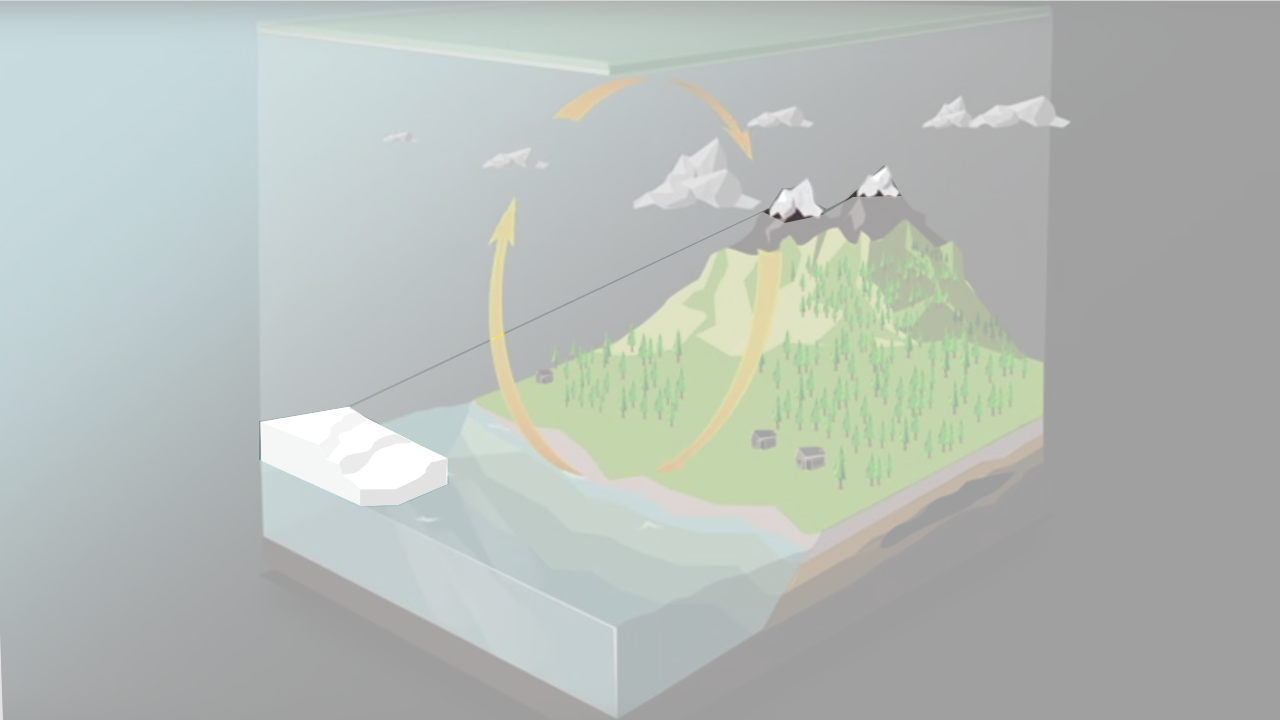
\includegraphics{bilder/WMO_Cycles_ice.png}
		\caption{Kryosphäre umfasst alle Formen und Schnee und Eis}
	\end{figure}
	\note{
		\begin{itemize}
			\item[] Eismassen stellen nach den Ozeanen die zweitgrößte Komponente des Klimasystems dar.
			\item[] das liegt an der Wärmekapazität von Wasser und seinem Volumen
      \begin{itemize}
        \item[] Wasser: \SI{4,2}{J \per g \per K} bei \SI{20}{°C}
        \item[] Gestein etwa: \SIrange{0,7}{1}{J \per g \per K}
      \end{itemize}
      \item[] ca. 2\,\% des Wassers ist in fester Form in Gletschern und an den Polkappen dauerhaft gebunden.
  %		\item  inländische Eisflächen speichern ca. 75\% des globalen Süßwassers
  		\item[] Eis reflektiert die ankommende Sonnenstrahlung zu großen Teilen
  		$\rightarrow$ \textbf{\textcolor{blue}{Albedo-Effekt}}\\

  		\item[] Je weniger Eismassen, desto weniger Strahlung wird reflektiert und bleibt in der Atmosphäre $\rightarrow$ Verstärkung des Treibhauseffekts

  		\item[] Durch Rußablagerungen auf den Eismassen wird mehr Sonnenstrahlung absorbiert ("Black Carbon")
  		 $\rightarrow$ Schmelzen des Eis und Verringerung des Albedo-Effekts % (Nature Geoscience, 2014; doi: 10.1038/ngeo2180)
		\end{itemize}
	}
\end{frame}


\begin{frame}
	\frametitle{Kryosphäre - Komponenten}
	Die größten Komponenten der Kryosphäre sind:
	\begin{itemize}
		\item Meereis: schwimmende Eismassen, 19-27 Mio. km$^2$
		\item Eisschilde: über Grönland und der Antarktis, 14 Mio. km$^2$
		\item Permafrost: gefrorene Böden, 22,8 Mio. km$^2$
	\end{itemize}

	\glqq Ein einmal eingesetzter Rückzug großer kontinentaler Eisschilde kann selbst nach Stabilisierung der Randbedingungen [(CO$_2$-Emissionen)] über ein Jahrtausend lang anhalten\grqq{} (Latif, 2009 und IPCC, 2001)\\
	%$\rightarrow$ siehe auch: Trägheit des Klimas in Abbildung \ref{fig:traegheit}

	\note{
		\begin{itemize}
			\item[] Meereis flächenmäßig sehr groß, aber Volumen der Eisschilde deutlich größer
			\item[] Eisschilde durchschnittlich 1,7-2 km dick
			\item[] weitere Elemente:
			\item[] Schneebedeckung variiert jahreszeitlich besingt zwischen 2 und 45 Mio. km$^2$
			\item[] Gletscher bilden 'nur' 0.5 Mio. km$^2$
		\end{itemize}
	}
\end{frame}

\begin{frame}
	\frametitle{Meereis} % Bild -> Pexels Andrea Schettino
  \begin{columns}
    \column{.3\linewidth}
    \begin{figure}
      \centering
      \newlength{\imagewidth}
      \settowidth{\imagewidth}{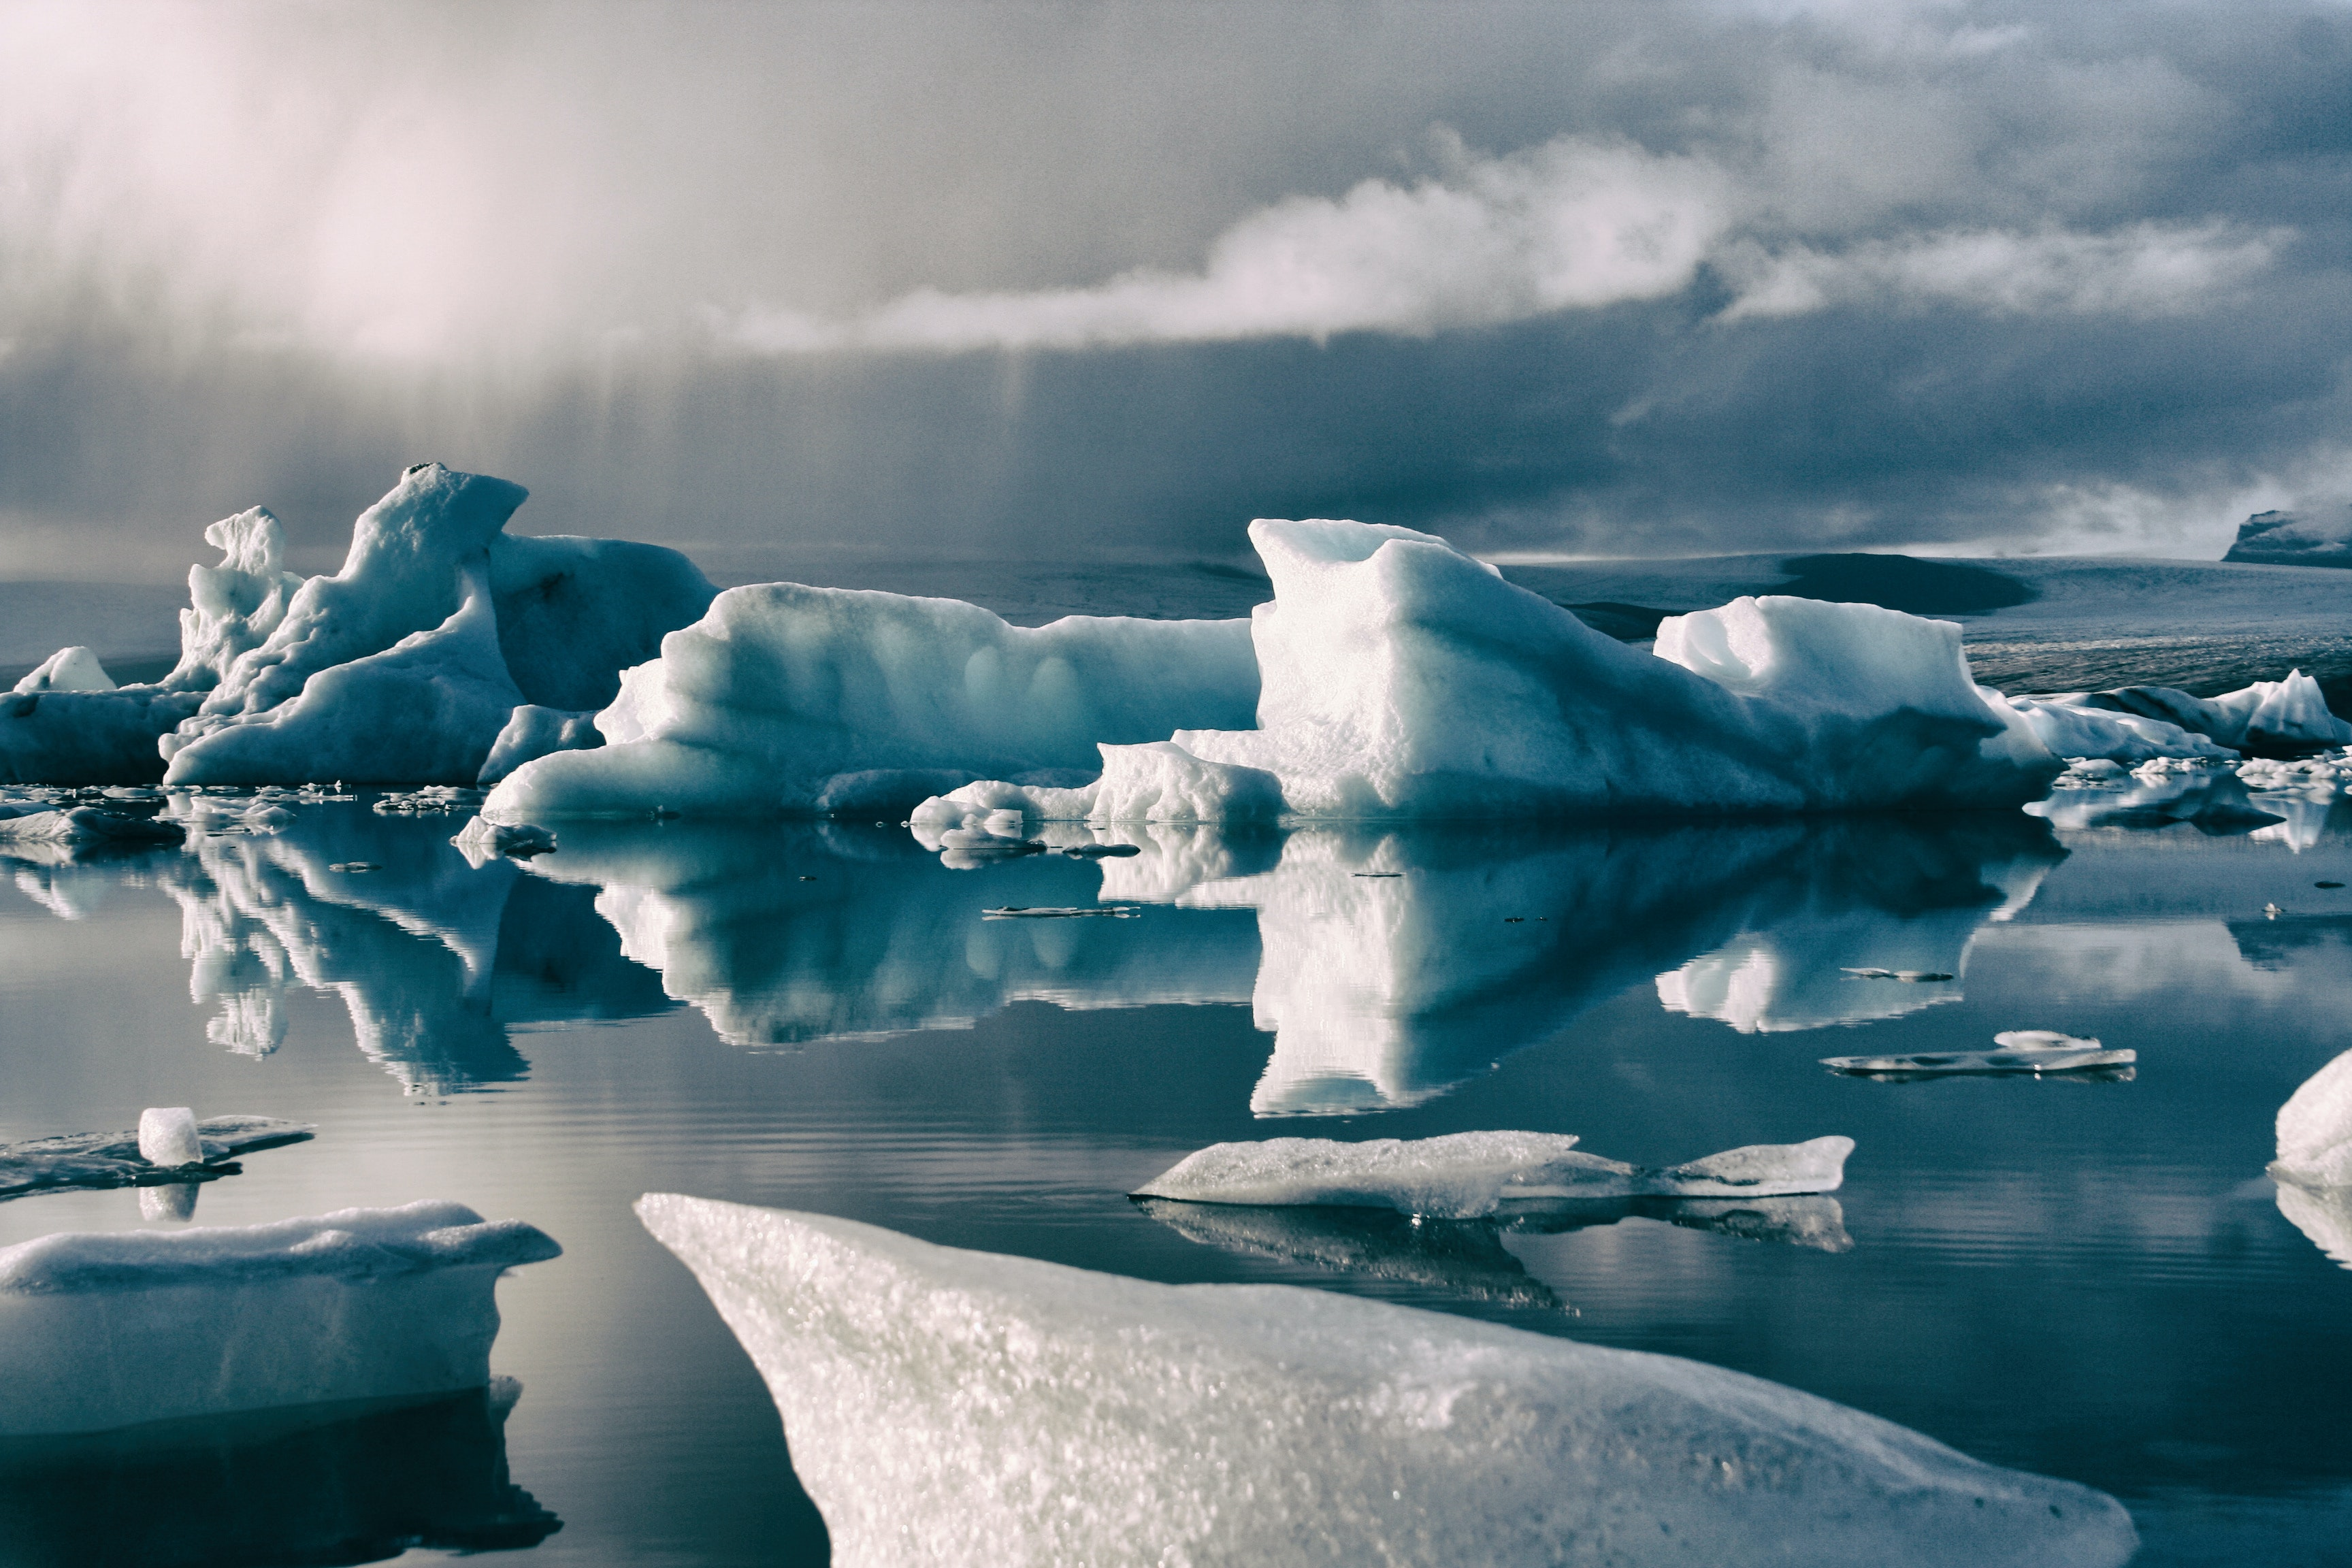
\includegraphics{bilder/ice-formation-in-body-of-water-3923277.jpg}}
      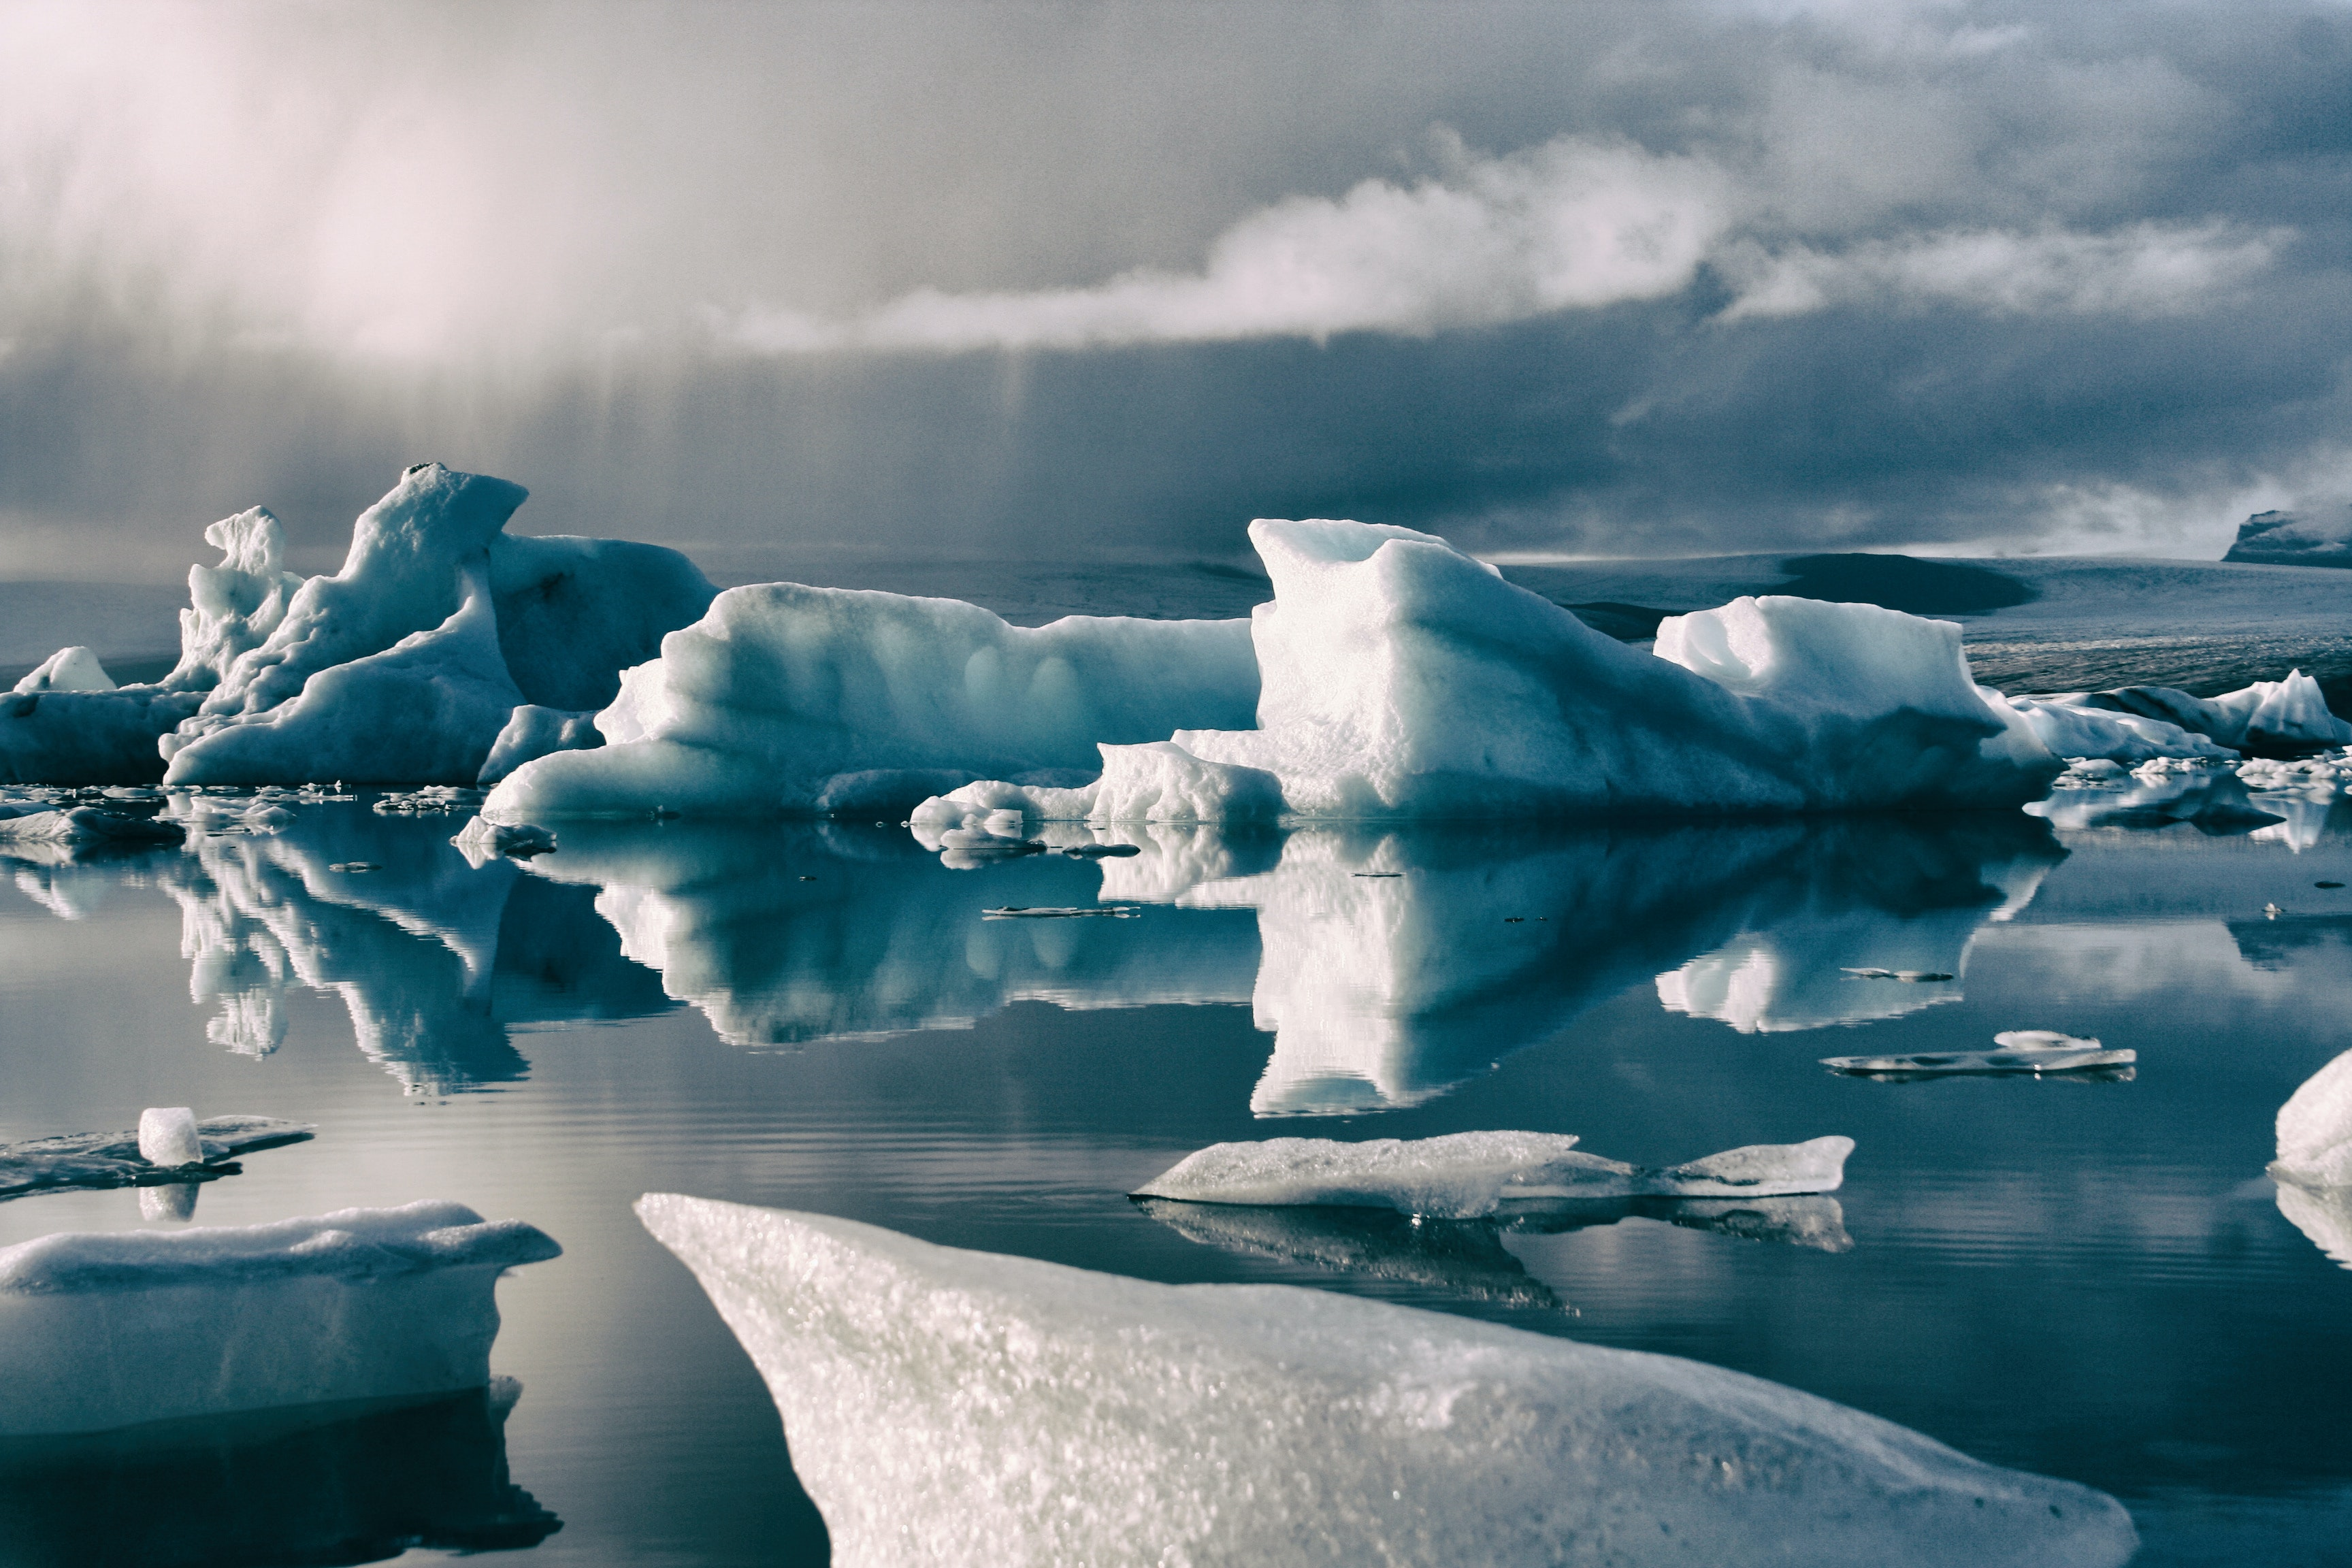
\includegraphics[trim=0 0 0.69\imagewidth{} 0, clip, width = 0.8\linewidth]{bilder/ice-formation-in-body-of-water-3923277.jpg}
      \caption{Quelle: Pexels, Andrea Schettino}
    \end{figure}
    \column{.7\linewidth}
	    \begin{itemize}
		    \item Bildet die Grenze zwischen Ozeanen und Atmosphäre
		    \item Luft über dem Meereis ist deutlich kälter als über dem Ozean
		    \item [$\rightarrow$] Abkühlung der Polarregionen und Verstärkung der atmosphärischen Zirkulation (Winde)
		    \item [$\rightarrow$] Beeinflusst Konvektion: je weniger Eis, desto schwächer die Konvektion, desto schwächer sind (langfristig) ozeanische Strömungen
	   \end{itemize}
   \end{columns}

	\note{
		\begin{itemize}
			\item[] Luft über dem Meereis ist deutlich kälter als über dem Ozean
			\item[$\rightarrow$] Wärmekapazität von Wasser, geringe Trägheit der Atmosphäre
			\item[] Winde entstehen zum Dichte-/Wärmeausgleich, stärkere Tmeperaturunterschiede führen also zu stärkeren Winden
			\item[] Konvektion beeinflusst vorallem die Tiefseestömungen
			\item[] Weniger Konvektion bedeutet auch weniger Nährstoffe in oberen Schichten der Ozeane
		\end{itemize}
	}
\end{frame}

\begin{frame}
	\frametitle{Eisschilde}
  \begin{columns}
    \column{.3\linewidth}
    \begin{figure}
      \centering
      \settowidth{\imagewidth}{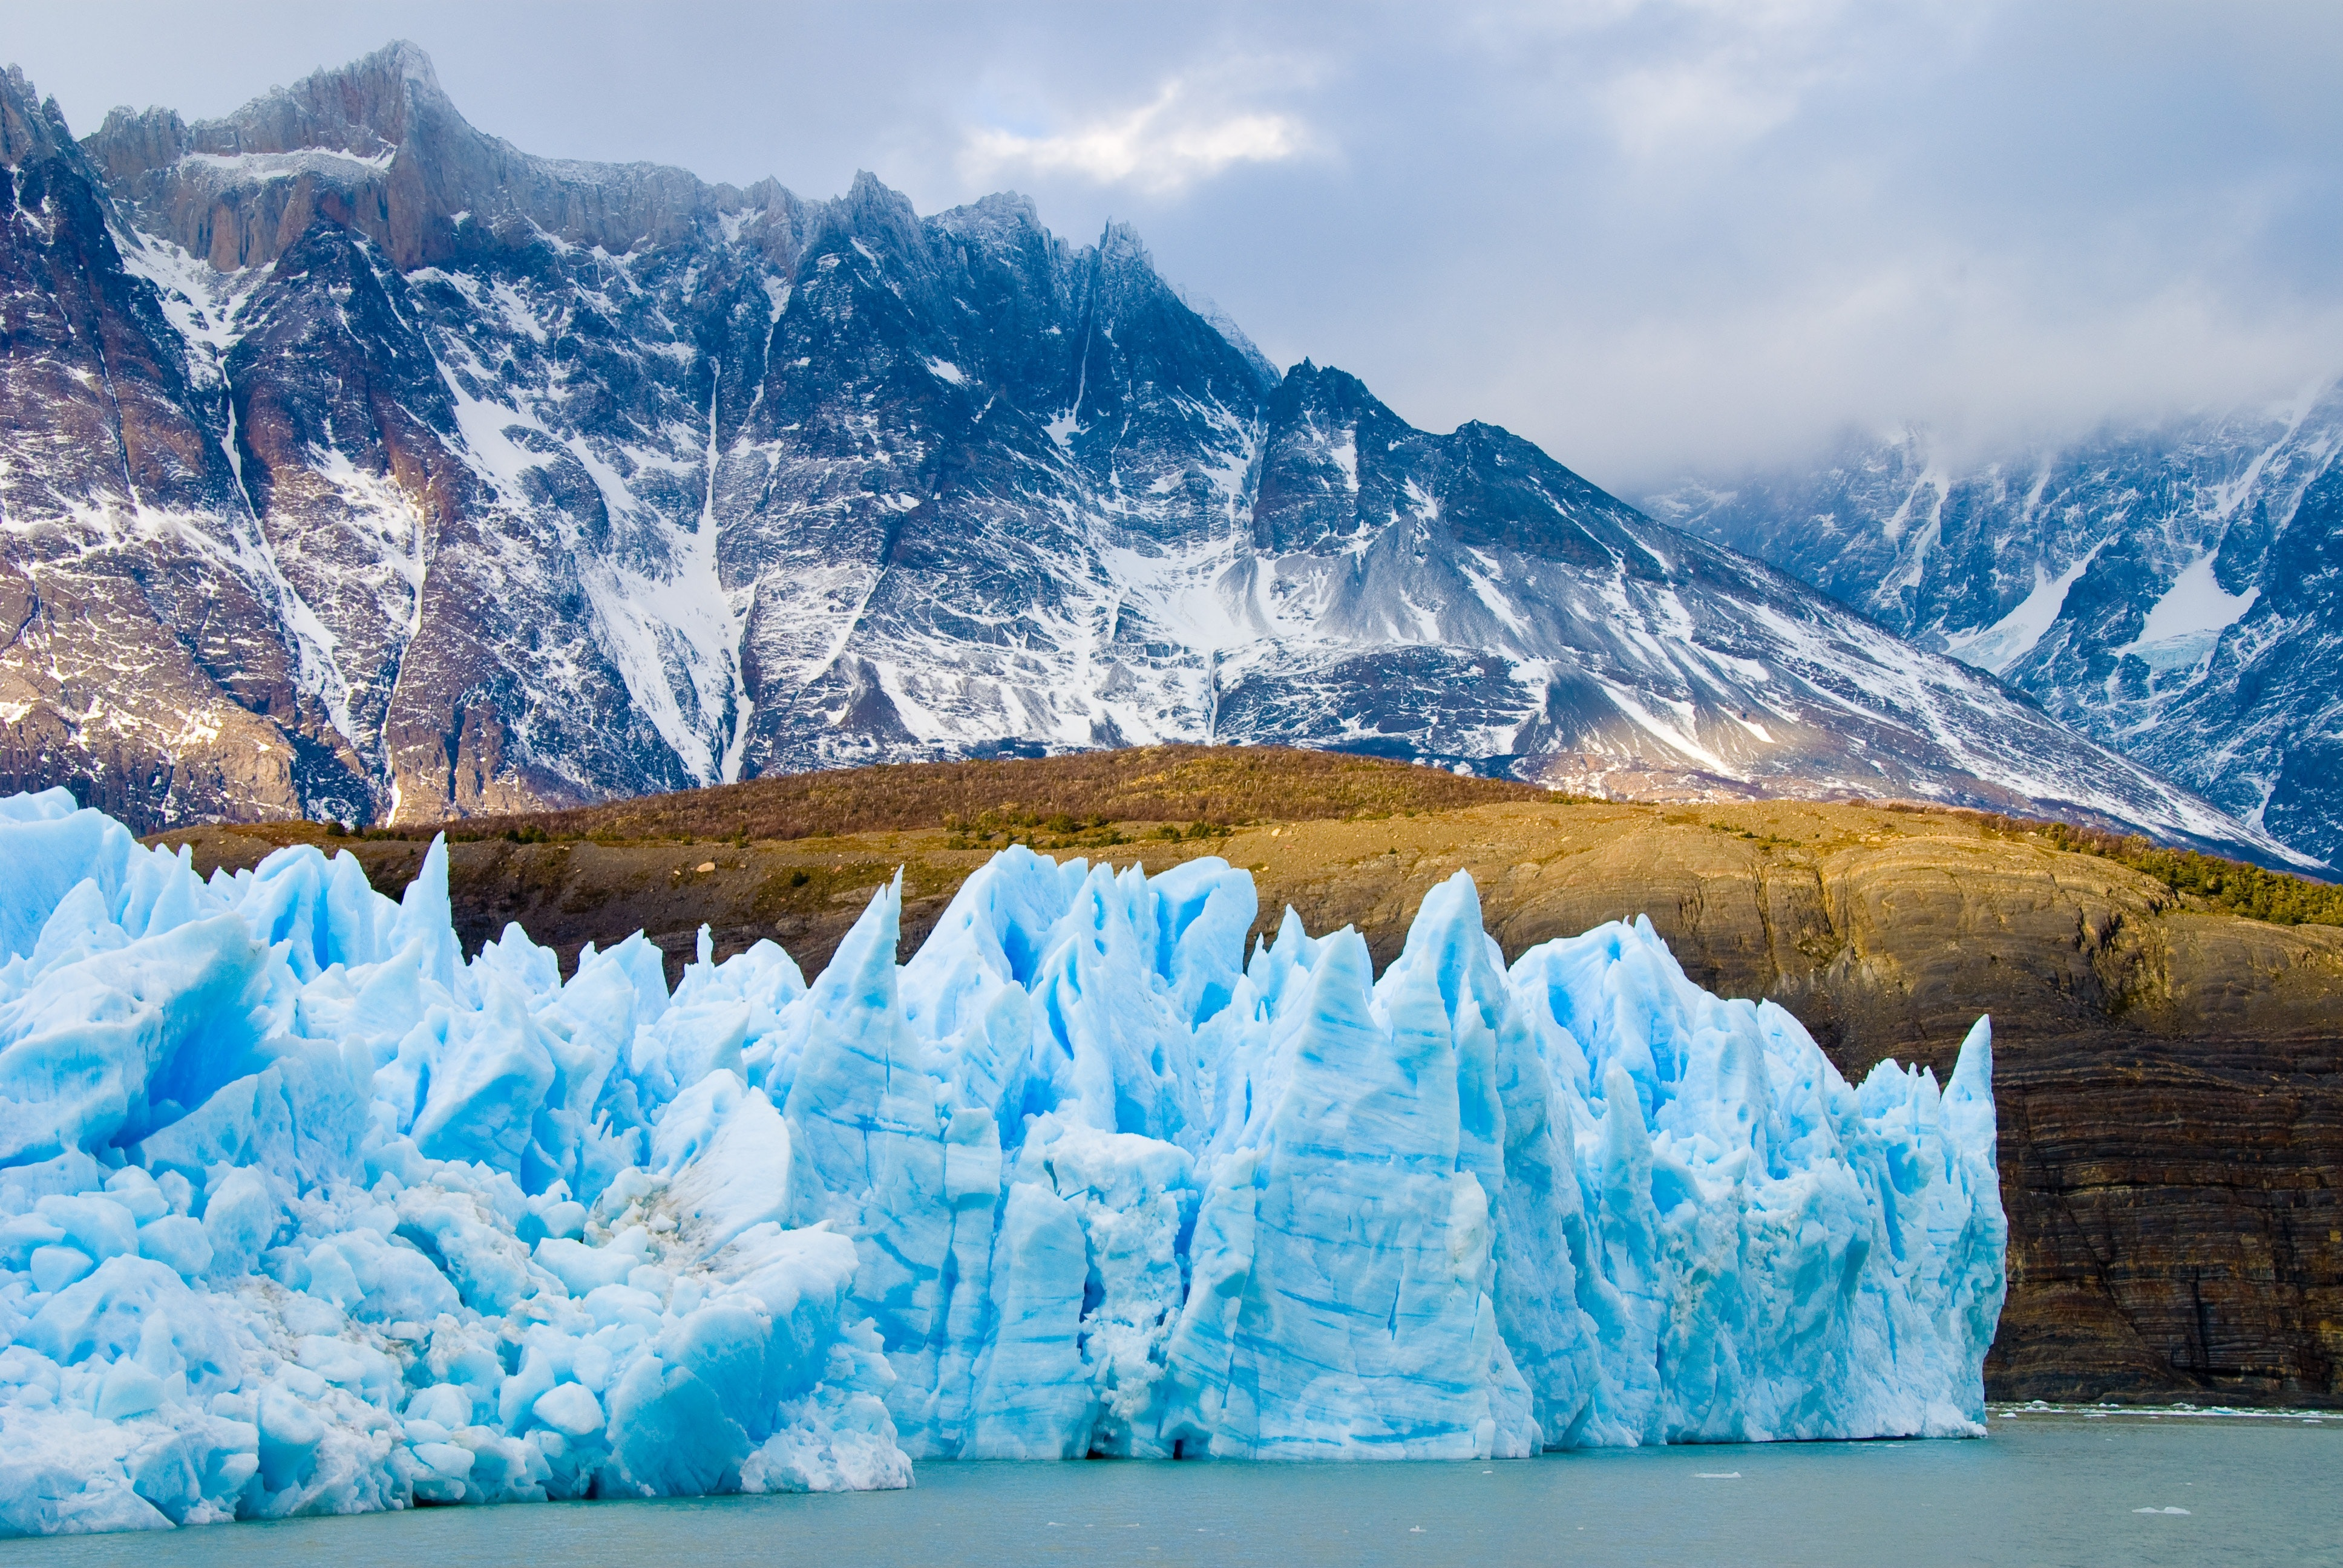
\includegraphics{bilder/panoramic-view-of-landscape-against-sky-255329.jpg}}
      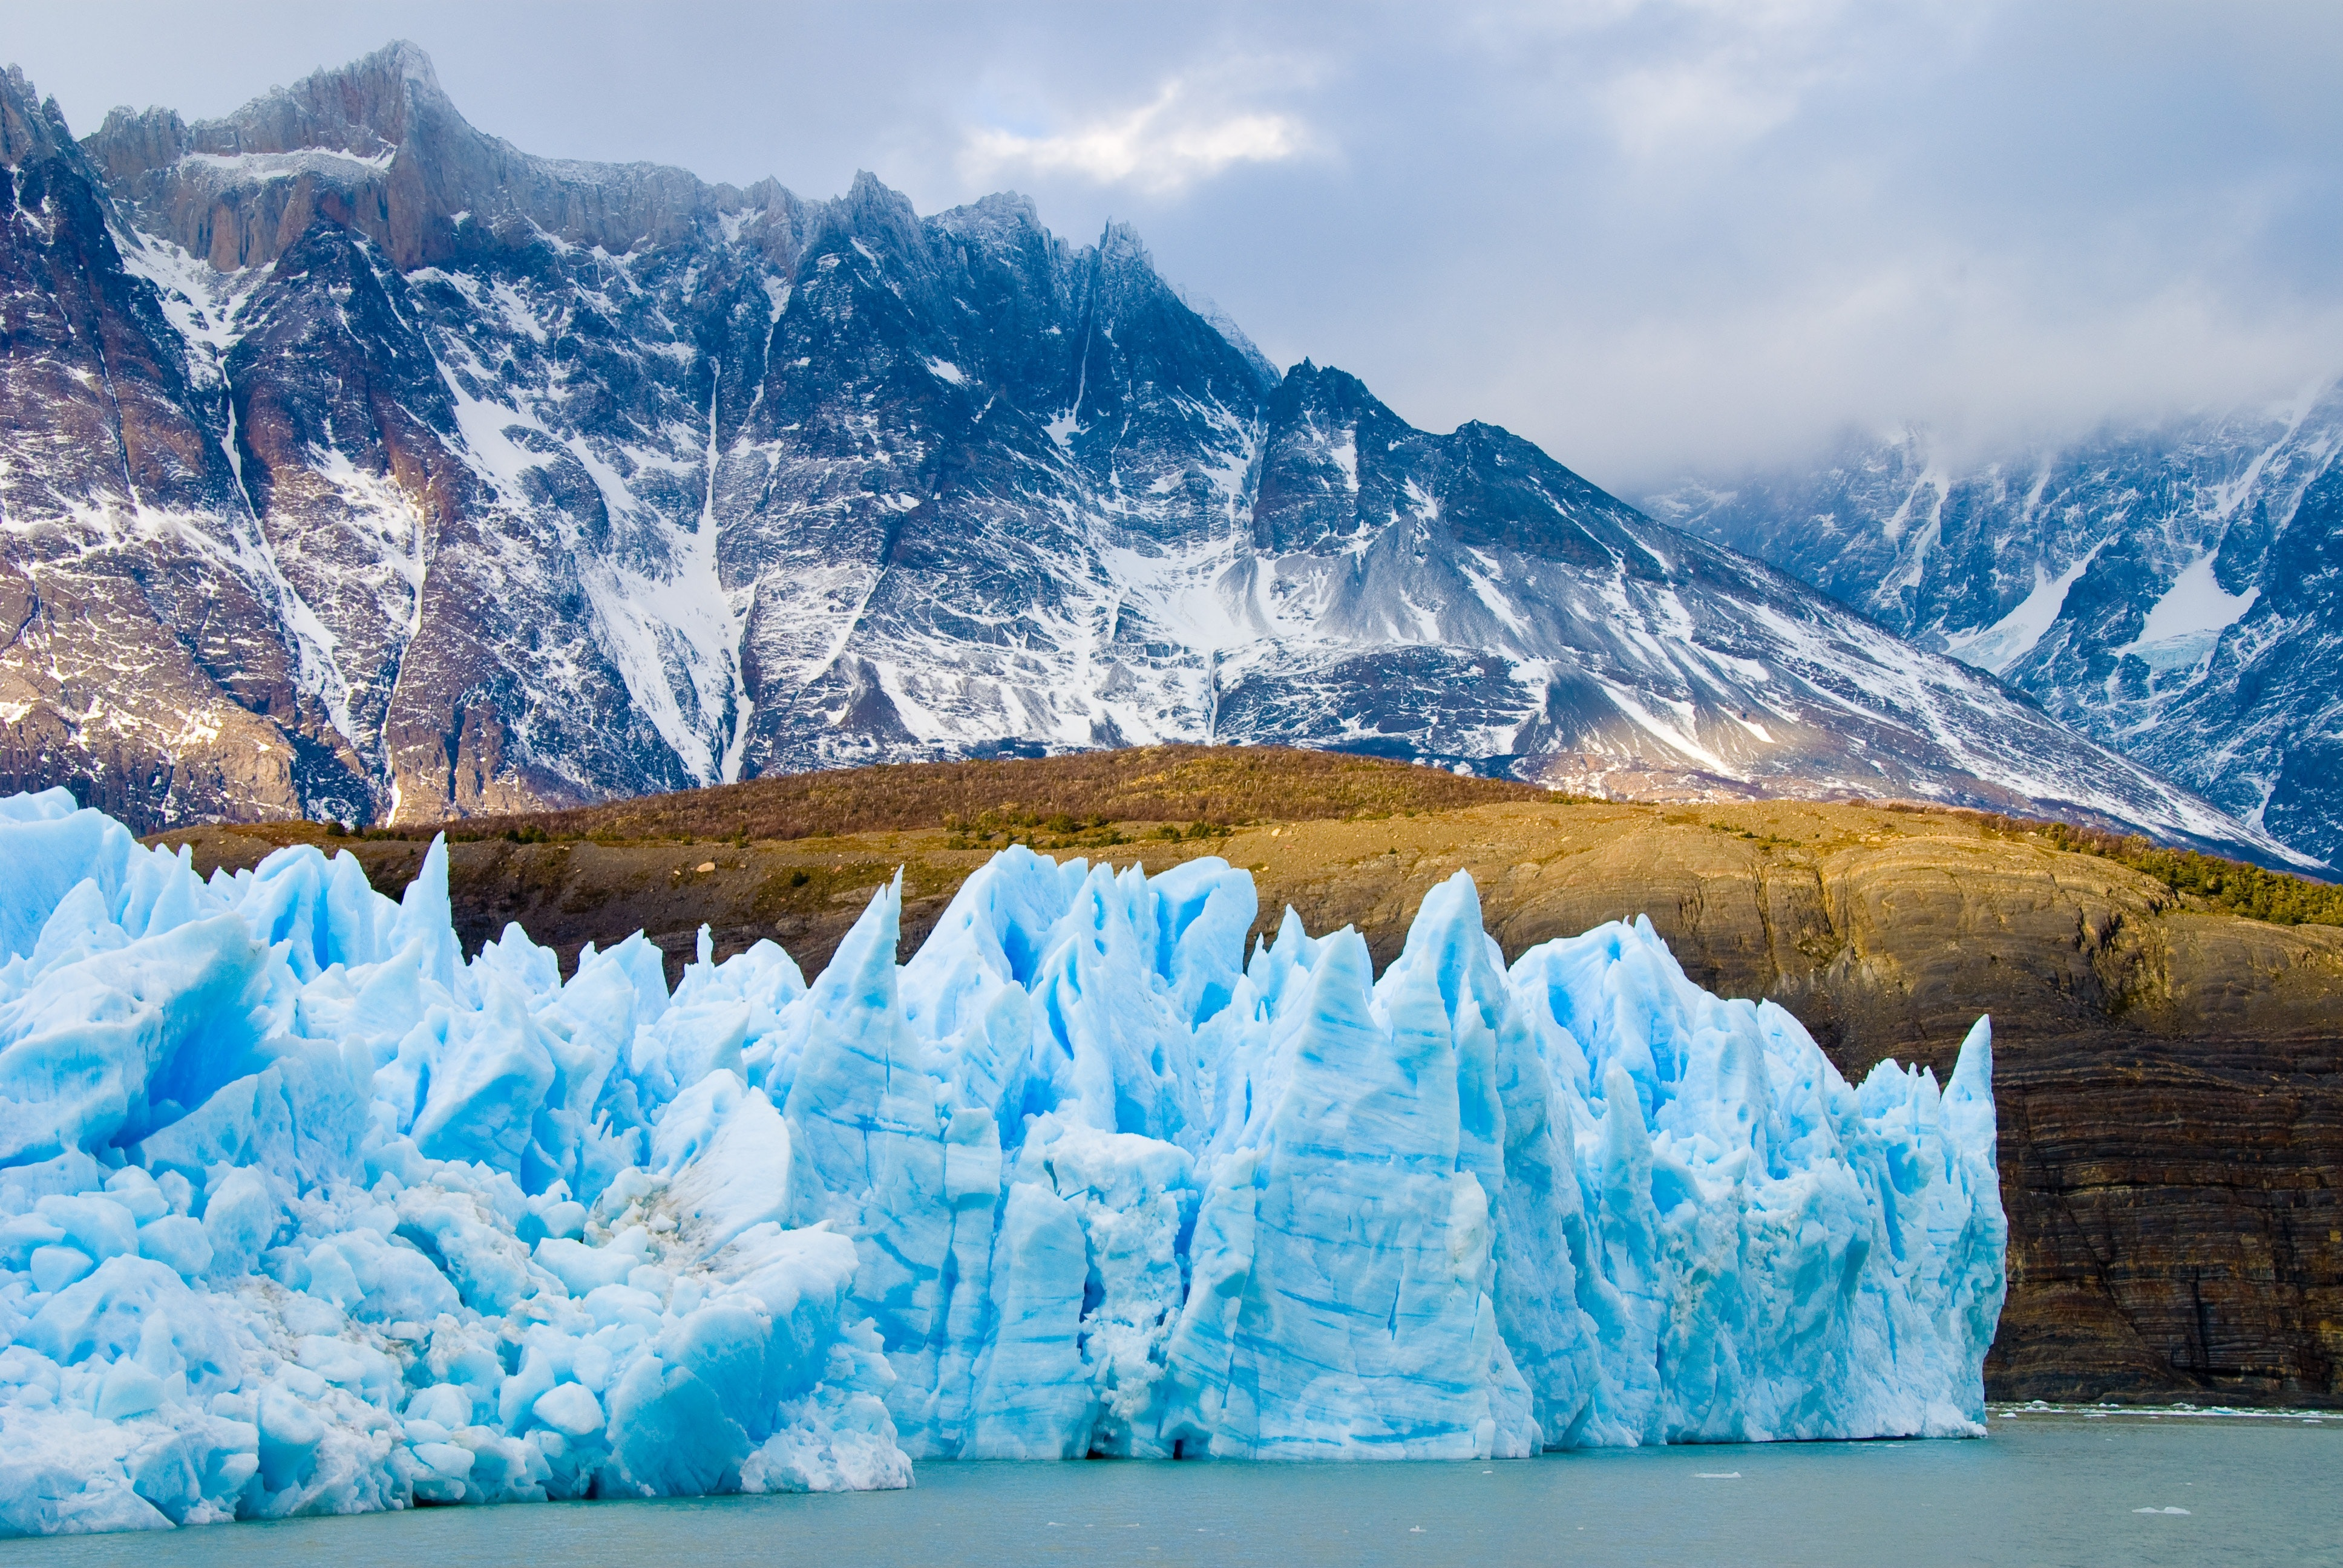
\includegraphics[trim=0 0 0.69\imagewidth{} 0, clip, width = 0.8\linewidth]{bilder/panoramic-view-of-landscape-against-sky-255329.jpg}
      \caption{Quelle: Pexels, Pixabay}
    \end{figure}
    \column{.7\linewidth}
	\begin{itemize}
		\item Volumen: 25 Mio. km$^3$ (Antarktis) + 3 Mio. km$^3$ (Grönland)
		\item Masse ist durch Niederschlag, Lufttemperatur und Strahlung bestimmt
		\item In der Antarktis gibt es Ausläufer des Landeises auf den Ozean hinaus (Schelfeis) $\rightarrow$ 0,7 Mio. km$^3$
%		\item tiefer liegende Schichten der Eisschilde schmelzen durch den Druck auf die Landmassen $\rightarrow$ erzeugt Spannungen im Eis
		\item Eisschilde schmelzen an randnahen Bereichen
		\item Höhere Temperaturen im Nordhalbkugelsommer gefährden das grönländische Eisschild besonders stark
		\item \textbf{Eisschilde haben das größte Potential für einen Anstieg des Meeresspiegels, da sie nicht -- wie das Meereis -- zum Meeresspiegel beitragen}
	\end{itemize}
  \end{columns}

	\note{
		\begin{itemize}
			\item[] Je mehr Schnee und je kälter, desto mehr Eis kann dich bilden
			\item[] Schelfeis zählt nicht zum Meereis, da es fest mit den Eisschilden verbunden ist
			\item[] Schelfeis bildet sich v.a. in Buchten, die von Eisschild umgeben sind
			\item[] Grönland besitzt quasi kein Schelfeis, daher schmilzt in Grönland direkt das Eisschild
			\item[] Der Antarktische Eisschild ist durch das Schelfeis etwas mehr geschützt
			\item[] Ein komplettes Abtauen der Eisschilde kann den Meeresspiegel bis zu 64 Meter ansteigen lassen. $\rightarrow$ sog. Meeresspiegel-äquivalent nach IPCC 2007
		\end{itemize}
	}
\end{frame}

\begin{frame}
	\frametitle{Permafrost}
  \begin{columns}
    \column{.3\linewidth}
    \begin{figure}
      \centering
      \settowidth{\imagewidth}{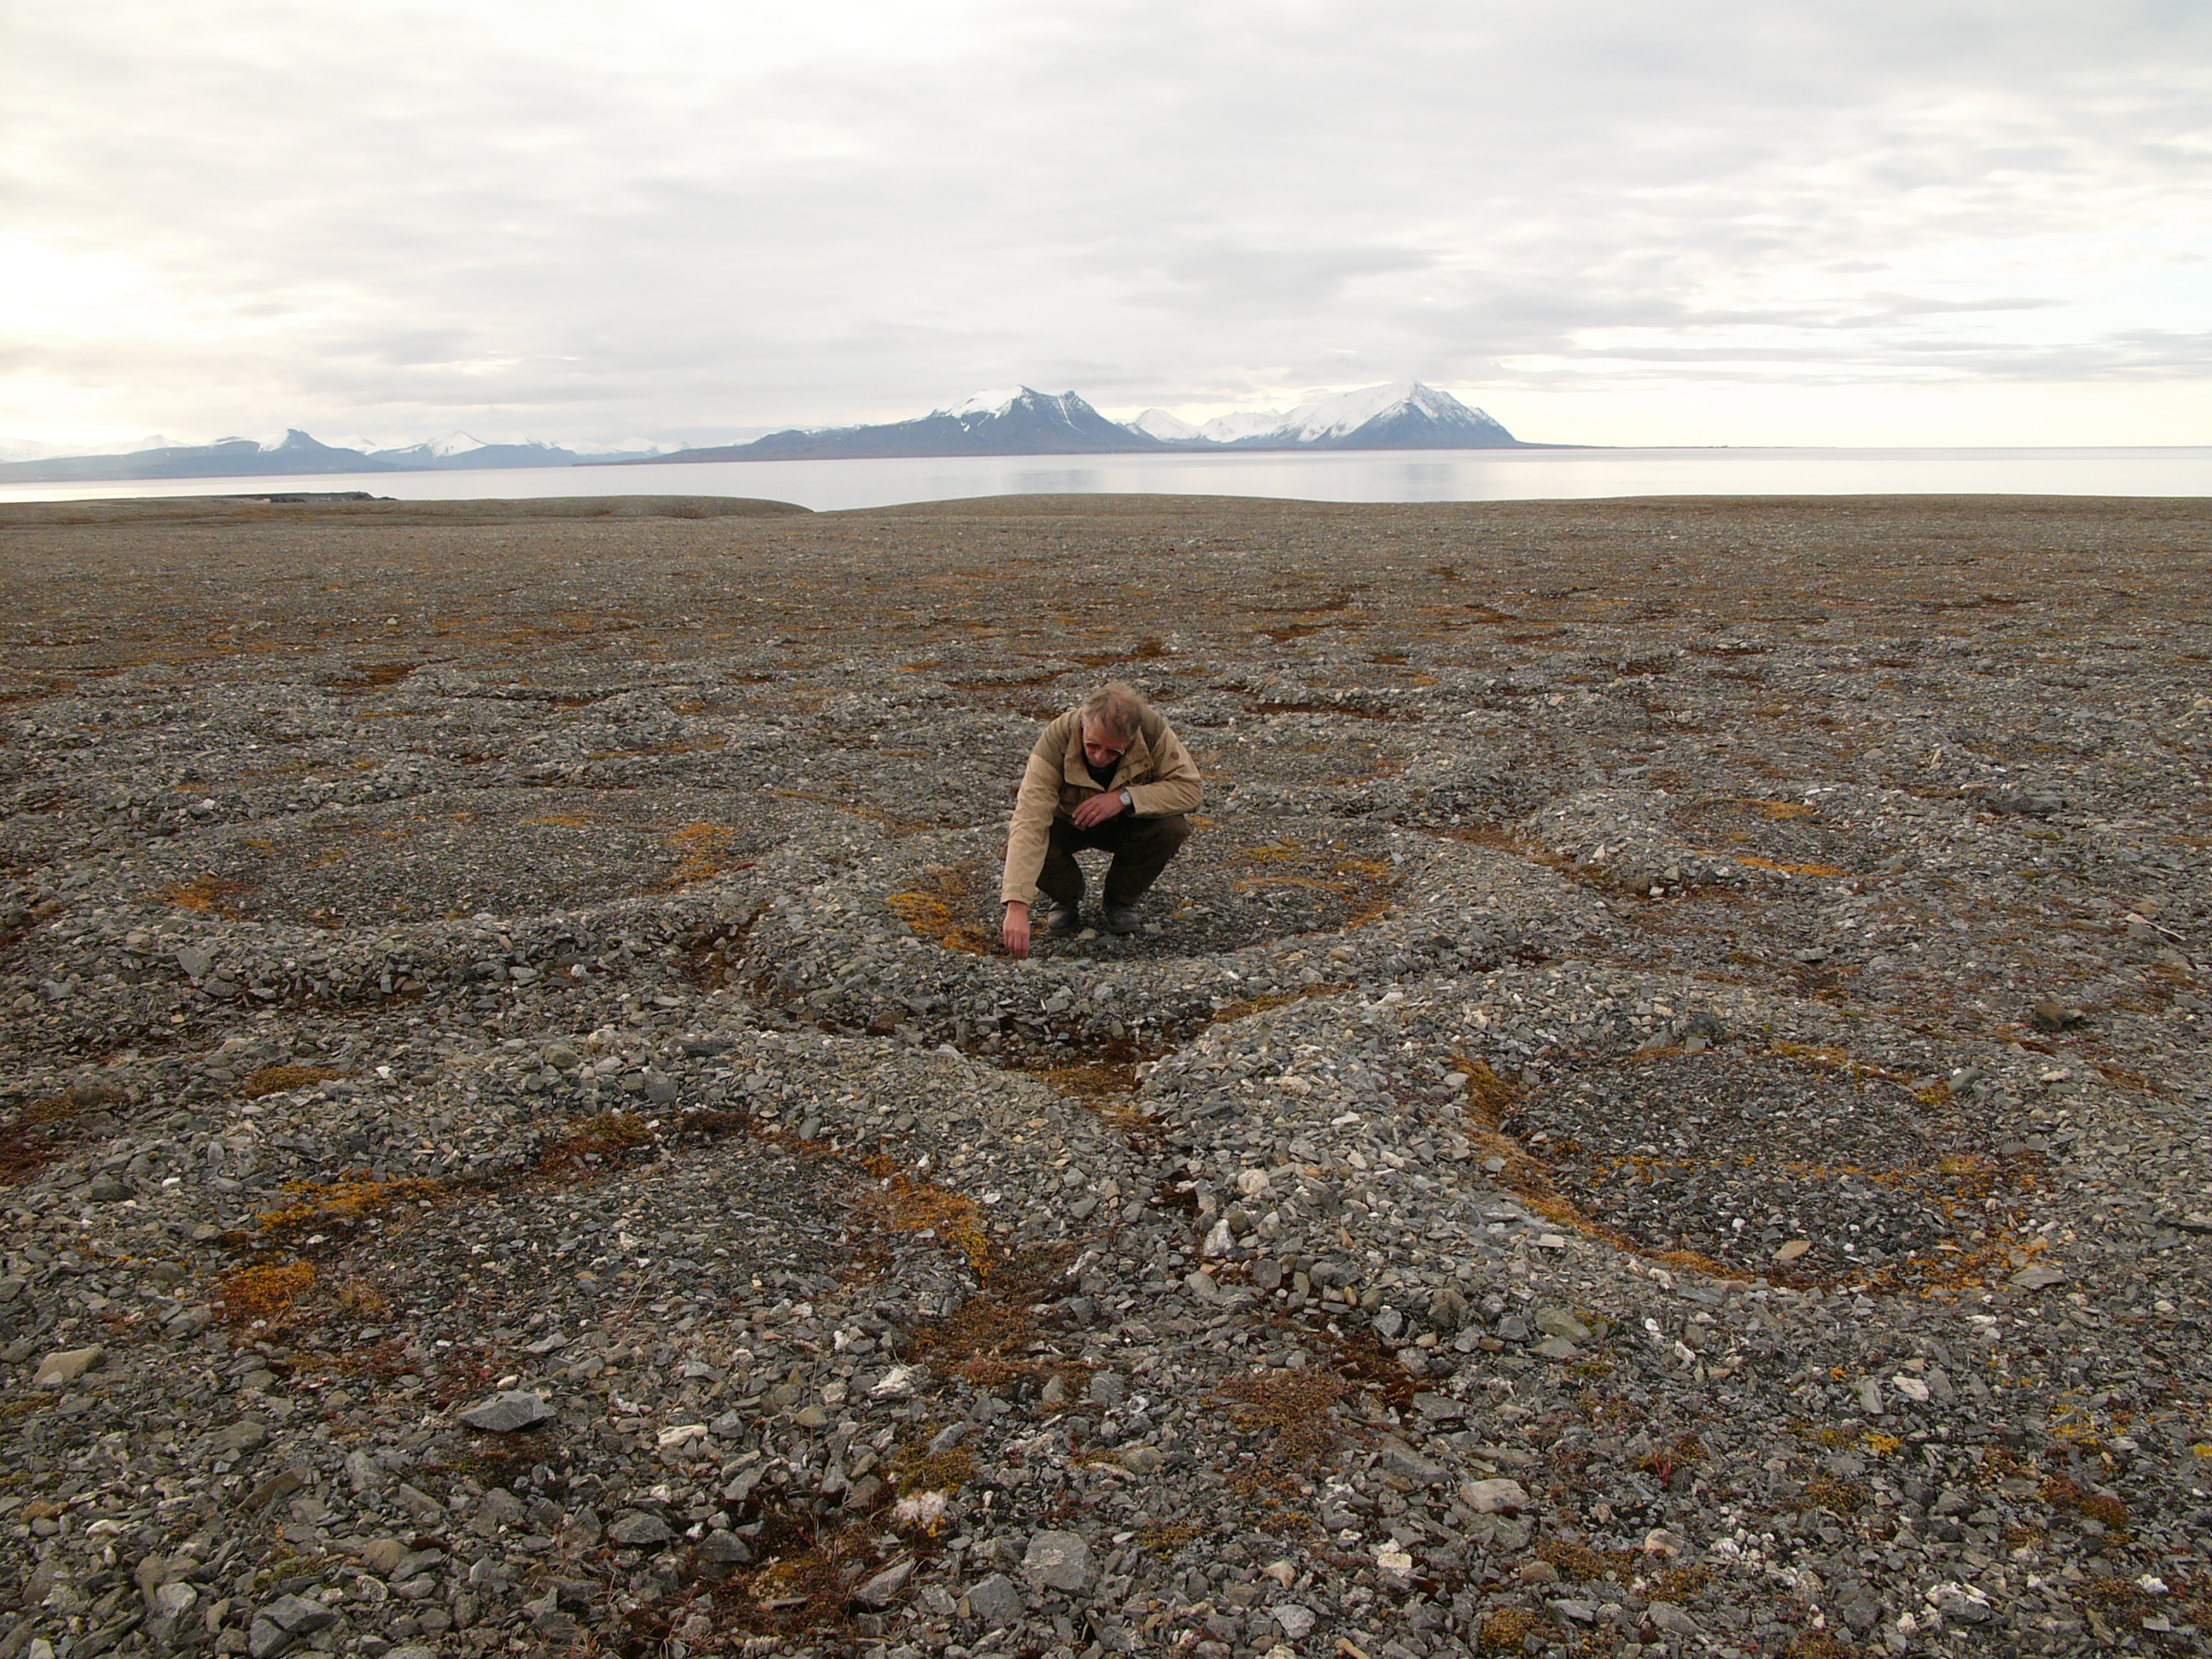
\includegraphics{bilder/Permafrost_stone-rings_hg.jpg}}
      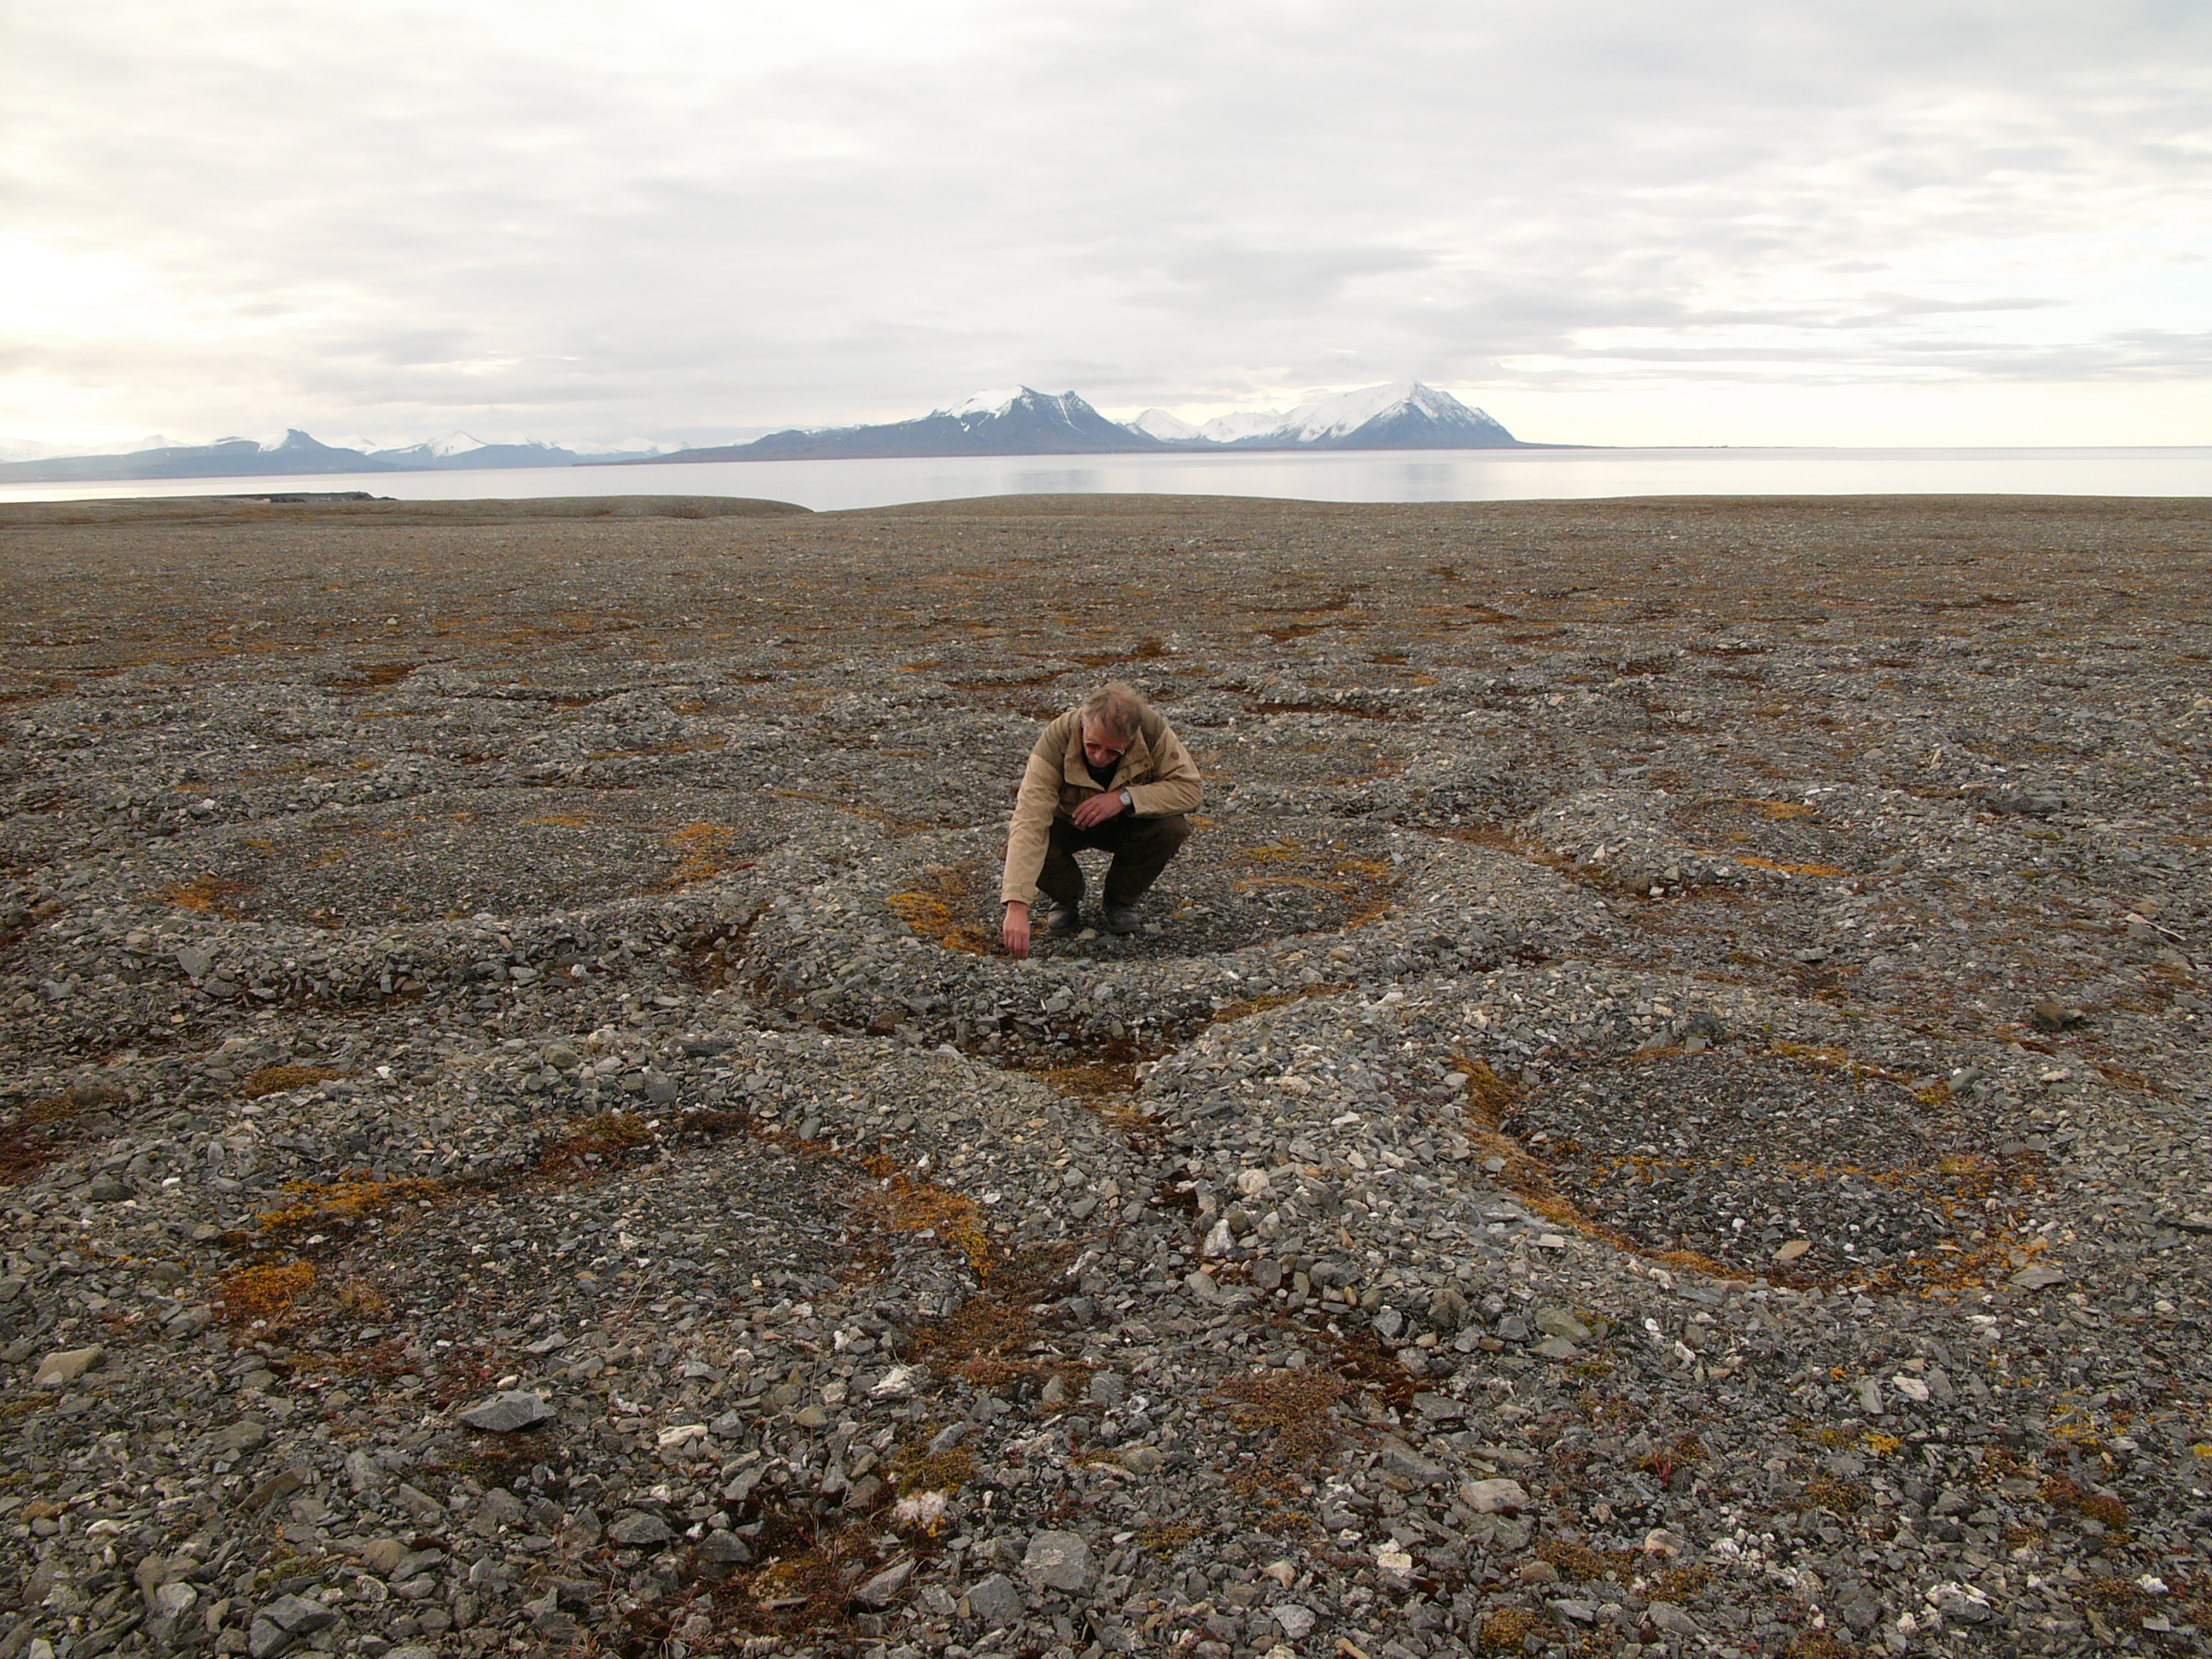
\includegraphics[trim=0 0 0.66\imagewidth{} 0, clip, width = 0.8\linewidth]{bilder/Permafrost_stone-rings_hg.jpg}
      \caption{Quelle: Wikimedia, Hannes Grobe}
    \end{figure}
    \column{.7\linewidth}
	\begin{itemize}
		\item Dauerhaft gefrorene Böden (permanent $<$ \SI{0}{°C})
		\item Größtenteils in Nordamerika und Eurasien
		\item Konserviert unzersetzte organische Materie
		\item [$\rightarrow$] Geschätzt 1000 Gt (1 Gt = $10^{15}$ g) Kohlenstoff gespeichert
		\item Deutliche Verschiebung der Permafrostgrenze im letzten Jahrhundert beobachtet
		\item Die globale Erwärmung gefährdet den Fortbestand des Permafrostes
		\item Folgen des Abtauens: Absenken der Böden, Überschwemmungen, Zersetzung bisher konservierter Materie
    \begin{itemize}
      \item[$\rightarrow$] Freisetzung großer Mengen CO$_2$ und Methan
    \end{itemize}
	\end{itemize}
\end{columns}

	\note{
		\begin{itemize}
			\item[] Frostmusterboden auf Grund von vor allem thermischer Kontraktion (Frosthub)
			\item[] Tiefe des Permafrostes ist abhängig von Oberflächen-Temperatur
      \item[] Zum Teil mehrere hundert Meter tief gefroren
			\item[] In Sibirien liegt kaum Schnee, sodass die Böden noch kälteren Temperaturen ausgesetzt sind
			\item[] Verschiebung der Permafrost-Grenze in Kanada z.B um \SI{100}{km} nach Norden im letzten Jahrhundert
			\item[] Absinken gefährdet auch lokale Infrastruktur wie Straßen, Städte und Öl-Pipelines
			\item[] Überschwemmung gefährdet Wälder $\rightarrow$ 'ertrinken'
      \item[] Wissenschaft nimmt an, dass deutlich mehr Treibhausgase freigesetzt werden, als die erwartete neue Vegetation binden würde
		\end{itemize}
	}
\end{frame}
